\documentclass[12pt]{report}
\usepackage{titling}
\usepackage{geometry}
\usepackage{graphicx}

\geometry{margin=1in}
\begin{document}
\title{Homework 3\\ \vspace{2 mm} {\large CS 383: Software Engineering}}

\author{32 Pounds}
\date{\today}
\maketitle
\clearpage

\chapter{Combat}
\textbf{Jordan Lynn, Derek Snyder} \\
Summary: When any player or NPC is fighting one another.\\
    
    Steps:
    \begin{enumerate}
        \item Intiation or Agro.
        \item Cool down on current attack begins.
        \item Damage is taken and delt, totals for these values are deducted from health.
        \item If either player or NPC has zero health the combat ends.
    \end{enumerate}
    
    \section{Intiation and Agro}
    Summary: Player strikes other party to begin combat or agro, when the player becomes too close to an agressive NPC.\\
    Preconditions: Two parties are within striking distance of each other. % Look into map/movement for intiation.
    
    \section{Cooldown}
    Summary: The minimum amount of time a player must wait after using an weapon/ability again. The duration of cooldown is based off of the weapon/ability used..\\ % See weapon swapping
    Preconditions: Player has used an weapon/ability.\\
    
    \begin{enumerate}
        \item Cooldown starts.
        \item Cooldown ends after preset amount of time.
    \end{enumerate}
    Alternative: Player swapped weapon/ability while cooldown was active, thus reseting cooldown. \textit{See weapon swapping.}

    \section{Damage}
    Summary: The amount of hitpoints to decrement from the player or NPC's health. This varies between weapons and abilities.\\
    
    Preconditions: Stike must have landed on target.
    
    Alternative: The attack does not hit the intended target and instead misses.\textit{See Missing.}
    
    \section{Missing}
    Summary: When a player launches an attack and the attack doesn't land on the target.\\
    
    Preconditions: The player must have intiated an attack or as been attacked through agro.\\
    Alternative: The attack lands on intended target. \textit{See Damage}

    \section{Diagram}
    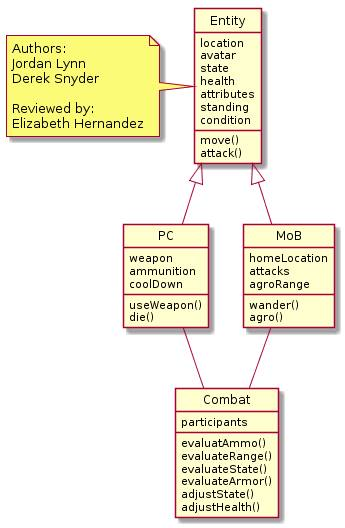
\includegraphics[width=\textwidth,height=\textheight,keepaspectratio]{combat.jpg}
\chapter{Player Class Summary}
 Upon starting the game, the user is assigned a base character(sales) for level 1 (training). After completion of level 1 the user may now choose between the following class of characters: Accountant(Heavy) -- IT(Distance) -- HR(Mage) -- Sales (Base).  Every class has four attributes with one attribute that caters specifically each class.\\ 
\begin{itemize}
\item \textbf{Strength} which is specialized to Accountants\\ 
\item \textbf{Speed} which is specialized to Sales\\ 
\item \textbf{Focus} which is specialized to IT\\ 
\item \textbf{Synergy} which is specialized to HR\\  
\end{itemize}
Specialization to each character makes upgrading attributes cheaper/easier for that character.\\

\textbf{\large{Accountant}}
\begin{itemize}
  \item Weapon: Roll of Quarters
  \item Miss percent: Constant with specialization -- High miss percentage with non-specialization weapon
  \item Cooldown Time: Standard (1 second) -- lowers with level increase % see player use cases
  \item An increase in Power Attribute -- Increase in Strike damage \\
\end{itemize}

\textbf{\large{IT}} 
\begin{itemize}
  \item Weapon: Floppy Disc Toss
  \item Miss percent: Low with specialization - High miss percentage with non-specialization weapon
  \item Cooldown Time: Average (1.5 seconds) -- lowers with level increase
  \item An increase in Focus Attribute -- Increase in disc toss accuracy (miss percent lowers)\\
\end{itemize}

\textbf{\large{HR}}
\begin{itemize}
  \item Weapon: Wand Pen (Spells)
  \item Miss percent: Constant with specialization - High miss percentage with non-specialization weapon
  \item Cooldown Time: High (2 seconds) -- lowers with level increase
  \item An increase in Synergy Attribute -- Increase in spell duration\\
\end{itemize}

\textbf{\large{Sales}}
\begin{itemize}
  \item Weapon: Stapler
  \item Miss percent: Constant with specialization - high miss percentage with non-specialization 
  \item Cooldown Time: Low (.5 seconds) -- lowers with level increase
  \item An increase in Speed attribute -- decrease in cooldown time
\end{itemize}


\chapter{Bureaucracy - Positive and Negative Attention}
\textbf{Madeleine Brennan, Elizabeth Hernandez}

\textbf{Diagram:}
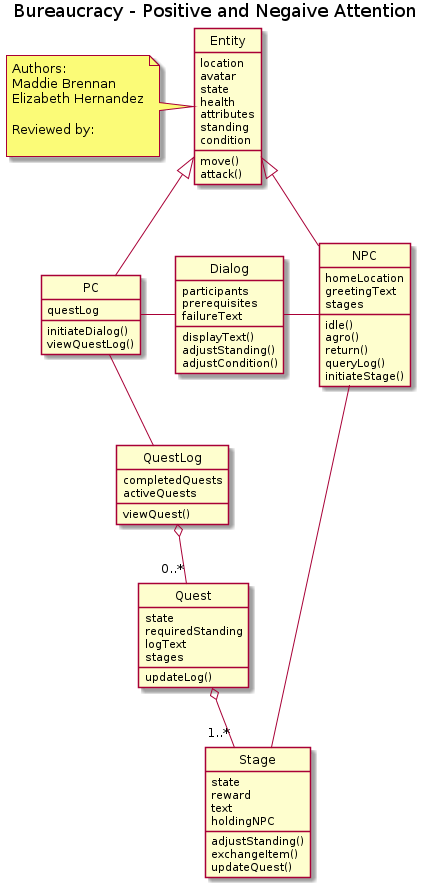
\includegraphics[width=\textwidth,height=\textheight,keepaspectratio]{Class_Diagram.png}\\

\textbf{Description:}

Bueracracy deals with interactions between entities in the game, with the biggest interaction within this catagory being quests. The diagram above visually shows the classes that are related to receiving and completing quests. This relates to bueracracy because completing quests will help achieve higher approval ratings with the faction that hosts the quest.

The root class is titled "Entity" and defines basic features of all characters in the game.
The classes "NPC" and "PC", which stand for "non-player character" and "player character" respectively, are extensions of the Entity class. 
Each PC will track the state of their quests in a Quest Log. 
The Quest Log will consist of 0 to many quests.
Each Quest consists of 1 to many quest Stages.
Stages hold requirements and rewards for each step of progression in its parent Quest.
Each Stage is held by an NPC.
A PC must engage in Dialog with an NPC in order to gain and advance through Stages of their Quests.

\chapter{Map and Movement}
\textbf{Brett Menzies, Gabriel Giovanini de Souze}

\textbf{diagram:}
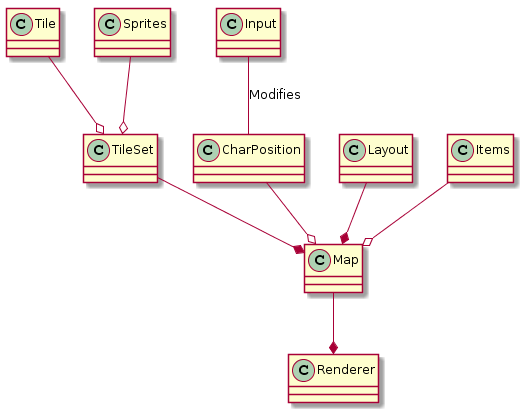
\includegraphics[width=\textwidth,height=\textheight,keepaspectratio]{map_and_movement.png}\\
\textbf{Description:}
The map subsystem revolves around the\`{ }Map'' class,
which is composed of a\`{ }Layout'' and a\`{ }Tileset'',
 and aggregates sets of ``Item Position'' and ``Player Position'' classes.
 A\`{ }Renderer'' class requires an instance of a\`{ }Map'';
  Its other connections are outside the scope of this diagram.
  A\`{ }Tileset'' aggregates ``Tiles'' (fixed size map tiles) and 
   ``Sprites'' (Other images drawn on a map, like items and characters) for use by the map and rendering code.
    Each ``Item position'' object represents the position and sprite id of items that have been dropped on the map.
    ``Character position'' acts similarly, except it can be modified by\`{ }input'', which represents 
     networked, npc, and local player inputs for the purposes of this diagram.

     \chapter{The Player}
     \textbf{Michael Mueller, Alexia Doramus}\\

     \noindent\textbf{Diagram:}\\
     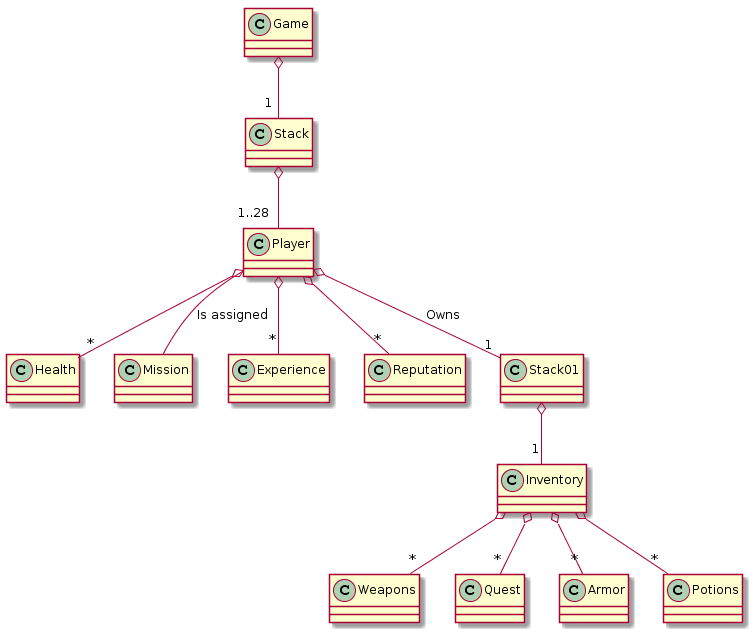
\includegraphics[width=\textwidth]{playerclass.png}\\

     \noindent\textbf{Description:}\\
     The player class is an aggregate of multiple parts. It consists of ``health'', ``experience'', ``reputation'', and it owns an ``inventory''. The player class can also be assigned a\`{ }mission''. The\`{ }inventory'' is part of a stack that keeps track of the multiple items, including: ``weapons'', ``quest items'', ``armor'', and ``potions''. The\`{ }player'' is part of a stack which can consist of up to 28 players. The stack that is an aggregation of the players is part of the game.


\end{document}
